
Si bien el fenómeno de resonancia magnética ha sido explotado durante más tiempo en el área de Química, particularmente mediante la espectroscopía (Capítulo \ref{chapter_espectro}), sin lugar a dudas fue la capacidad de realizar imagen la que revolucionó el campo de la Medicina, tanto en términos clínicos como en el área de investigación. Los métodos para producir imagen mediante el fenómeno de resonancia se gestaron de manera simultánea a la tomografía axial computarizada (TAC, ver Capítulo \ref{chapter_historia}) pero, aunque ambas técnicas comparten muchos conceptos, la manera en que se codifica la posición espacial en resonancia es bastante distinta a como lo hace la TAC, siendo la segunda más intuitiva por ser una simple retro-proyección o transformación de Funk-Radon. Las imágenes de resonancia magnética se obtienen mediante un proceso no necesariamente más complejo, pero sí menos amigable de primera instancia. 

Primero debemos considerar qué es lo que buscamos codificar. En términos prácticos, deseamos saber la relación espacial que guardan con el resonador y con nuestro paciente o muestra, las diferentes partes que lo componen, además de que explotemos los mecanismos de generación de contraste para distinguir entre ellos (Capítulo \ref{chapter_relajacion}). Como en todas las imágenes digitales, tendremos que dividir artificialmente nuestro objeto real (paciente o muestra) en un cierto número de elementos, cada uno denominado \index{pixel} \emph{pixel} (portmanteau de \emph{pic}ture-\emph{el}ement). En el caso que nos compete, buscamos mapear en dos dimensiones (imagen) algo que habita en un espacio tridimensional (paciente u objeto), por lo que cambiaremos el término pixel por \index{voxel} \emph{voxel} (\emph{vol}ume-\emph{el}ement). Es común, aunque no deseable, intercambiar ambos términos, siendo el preferido el término de voxel. Un voxel tiene entonces unas coordenadas y dimensiones en los ejes \textit{x}, \textit{y} y \textit{z}. Es una pequeña caja que contiene tejido, y por lo tanto, muchos átomos de hidrógeno; podemos imaginar cada voxel como tubos de ensaye con muestras, sobre las cuales queremos indagar parámetros claros, como la cantidad de H que contiene. Los métodos que se explican adelante están orientados a delimitar cada uno de estos voxeles, e interpretar la señal de resonancia magnética como proveniente de estas entidades discretas.

La herramienta que utiliza la codificación espacial es la dependencia lineal de la frecuencia de precesión $\omega$ con respecto al campo magnético \Bzero que experimentan los spins (Ecuación \ref{eq_Larmour}). Aprovechando esta relación tan simple, es posible alterar la frecuencia de precesión mediante modificaciones lineales del campo magnético principal utilizando electroimanes que se suman o restan a \Bzero. A estos campos magnéticos secundarios les llamamos \index{gradientes|textbf} \emph{gradientes} (de campo magnético), y se logran mediante electroimanes resistivos, con el objetivo de prenderlos y apagarlos a voluntad, y están situados en el espesor del toroide del resonador (Figura \ref{fig:gradientes}).  Los gradientes producen campos en \Bzero de manera predecible, y con una magnitud mucho menor que el campo principal, siendo habitual en equipos modernos tener modificaciones en el orden de 20 a 80 mT/m. Es decir, por cada cm de distancia, el campo magnético se modifica entre 0.2 y .8 mT. Conociendo la amplitud de los gradientes ($G$), podemos predecir la frecuencia de precesión de spins ($\omega_i$) colocados en determinada posición espacial ($r_i$) mediante la modificación de la equación \ref{eq_Larmour}:

\begin{equation}
 \omega_i = \gamma(B_0 + G \cdot r_i)
 \label{eq_LarmorGradientes}
\end{equation}




\begin{figure}[htb]
 \begin{figg}
   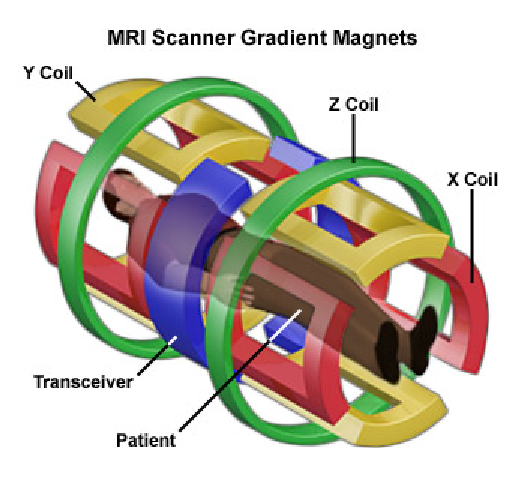
\includegraphics[width=0.7\textwidth]{gradientes}
   \caption{Configuración física de los gradientes de campo magnético. Las estructuras verdes, rojas y amarillas son en realidad conjuntos de cables por los que se pasa una corriente eléctrica, produciendo así un campo magnético secundario que se suma algebraicamente a \Bzero. Tomado de \url{https://nationalmaglab.org}.}
 \label{fig:gradientes}
 \end{figg}
\end{figure}




\section{Selección de rebanada (excitación selectiva)}
De las tres dimensiones que tenemos que codificar, la más sencilla es la que identificaremos como rebanada o corte del objeto. Cuando hablamos de cortes en humanos, consideramos los planos anatómicos clásicos: axial, coronal y sagital. Los cortes axiales atraviesan al sujeto de forma perpendicular a su eje longitudinal (superior-inferior); los coronales lo hacen perpendicular al eje antero-posterior, y los cortes sagitales son paralelos a la línea media. Por convención y por la manera en que la mayoría de los resonadores magnéticos de humanos están construidos, el eje longitudinal del paciente (habitualmente acostado) penetra el túnel del magneto, y se denomina el eje \textit{z}, siendo los ejes \textit{x} y \textit{y} perpendiculares a éste. Para fines didácticos, la mayoría de los ejemplos que se presentan en este capítulo tratan de rebanadas axiales (perpendiculares al eje \textit{z}), a menos que se especifique lo contrario. A partir de la ecuación \ref{eq_LarmorGradientes}, podemos excitar selectivamente a un grupo de spins mediante la aplicación de una radio-frecuencia (RF o \Bone) con un ancho de banda que coincida con las frecuencias de precesión de la zona de interés (Figura \ref{fig:rebanadas}). Recordemos que lograremos perturbar \Mz únicamente si la frecuencia de \Bone es igual a la frecuencia de precesión. Dada la presencia del gradiente del campo magnético, hemos manipulado estas frecuencias, y conocemos el rango (ancho de banda) en el que se encuentran, así que es fácil producir un pulso de RF que contenga las frecuencias calculadas. Todos los spins del cuerpo del paciente están precesando con cierta frecuencia, pero existe un sitio dentro del resonador donde hemos producido un rango de frecuencias específicas, y únicamente los spins en esta región serán perturbados mediante \Bone. Si utilizamos un pulso que desvíe 90\degrees a \Mz, entonces lograremos colocar la totalidad de la magnetización neta en el plano \textit{x,y} en una rebanada, mientras que esto no se logrará en spins que no estén en el sitio de interés.

Las rebanadas o cortes tienen un centro (posición) y un espesor. Estos pueden manipularse mediante tres parámetros: la frecuencia central, el ancho de banda, y la amplitud de $G$ mediante la siguiente relación:
\begin{equation}
 \Delta\omega = \gamma G \Delta{z}
\end{equation}
donde $\Delta\omega$ indica el ancho de banda de la RF, y $\Delta{z}$ indica el grosor de la rebanada. La orientación de $G$ determinará el tipo de corte: si el gradiente se aplica sobre el eje $z$, lograremos una rebanada axial, y si se aplica sobre el eje $x$ lograremos rebanadas sagitales. Es posible hacer cortes oblicuos utilizando trigonometría para usar de manera simultánea los tres juegos de gradientes. La frecuencia central identificará el centro de la rebanada en relación a la ecuación \ref{eq_LarmorGradientes}, mientras que el ancho de banda, en combinación con $G$, determinarán el espesor de la rebanada (Figura \ref{fig:rebanadas_BW}).


\begin{figure}[htb]
 \begin{figg}
   \includegraphics[width=\textwidth]{rebanadas}
   \caption{Excitación selectiva de una rebanada. Tomado de \cite{mcrobbie2007mri}.}
 \label{fig:rebanadas}
 \end{figg}
\end{figure}

\begin{figure}[htb]
 \begin{figg}
   \includegraphics[width=\textwidth]{rebanadas_BW}
   \caption{Control del grosor de la rebanada. La amplitud del gradiente (a) y el ancho de banda del pulso de RF (b) se utilizan para definir el espesor del corte. Tomado de \cite{mcrobbie2007mri}.}
 \label{fig:rebanadas_BW}
 \end{figg}
\end{figure}



\section{Codificación mediante frecuencia}
Una vez que se realizó una excitación selectiva de una rebanada, podemos codificar una de las dos dimensiones restantes mediante la frecuencia de precesión. Este proceso es sencillo, y nuevamente se basa en la frecuencia de Larmour, $\omega$, que depende directamente del campo magnético experimentado, que puede ser modulado linealmente mediante gradientes, tal como se describió en la ecuación \ref{eq_LarmorGradientes}. Imaginemos una imagen de tres pixeles, cada uno con una cantidad total de moléculas de agua, como se observa en la Figura \ref{fig:gradientes2}. Si aplicamos mediante un gradiente una modulación del campo magnético de izquierda a derecha (de 2.99 T a 3.01 T), los spins del cada pixel experimentarán diferentes campos magnéticos entre ellos, y por ende cada uno precesará a una frecuencia dada, que rondará entre 127.075 y 127.925 MHz. 
 
\begin{figure}[htb]
 \begin{figg}
   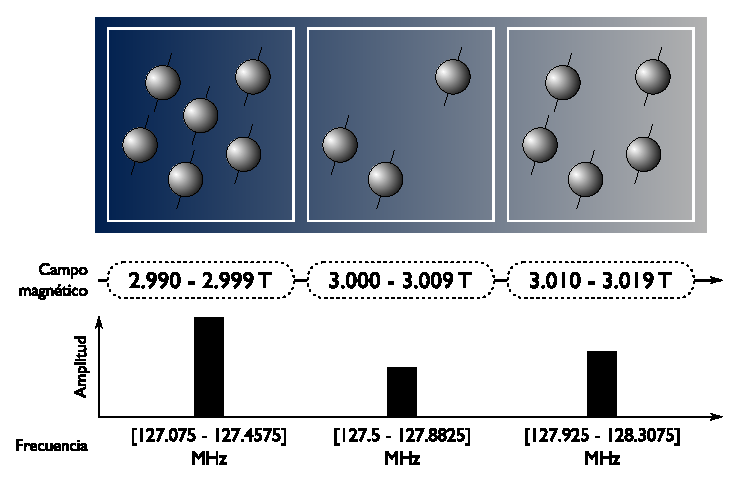
\includegraphics[width=\textwidth]{gradientes2}
   \caption{Codificación espacial mediante frecuencia.}
 \label{fig:gradientes2}
 \end{figg}
\end{figure}

Cuando recibamos la señal de resonancia proveniente de estos spins, ésta contendrá de manera simultánea las frecuencias en todo el rango antes mencionados, y cada frecuencia en este rango estará más o menos representada, dependiendo del número de spins que precesa a esa frecuencia. El ancho de banda que recibiremos está limitado por
\index{Ancho de banda|textbf}
\index{Bandwidth|textbf}

\begin{equation}
 BW = \gamma G (FOV).
 \label{eq_bw_read}
\end{equation}


Por supuesto, la división en tres pixeles es arbitraria y artificial, y la realidad es que se recibirá un enorme número de posibles frecuencias, pero todas ellas dentro del rango entre 127.075 y 127.925 MHz.  Si bien la señal recibida será altamente compleja, afortunadamente podemos analizarla utilizando uno de los tratamientos matemáticos más útiles de todos los tiempos: la transformada de Fourier. Formalmente, ésta postula que toda señal está en realidad formada por la suma de un número de señales periódicas de diferentes frecuencias y fases (Figura \ref{fig:Fourier_decomposition}). Es decir, la transformada de Fourier es como un prisma que descompone a la luz en sus coloridos componentes. A diario nos encontramos con aplicaciones de la transformada de Fourier, como en el ecualizador del sonido de un equipo de reproducción de música, que nos permite controlar la amplitud de rangos de frecuencias organizados en distintas bandas, desde las frecuencias más bajas a la izquierda, hasta las más altas a la derecha (Figura \ref{fig:equalizer}). 

\begin{figure}[htb]
 \begin{figg}
   \includegraphics[width=0.7\textwidth]{Fourier_decomposition}
   \caption{Transformada de Fourier. La curva compleja de color añil puede ser formada mediante la suma de las primeras tres curvas simples sinusoidales.}
 \label{fig:Fourier_decomposition}
 \end{figg}
\end{figure}

\begin{figure}[htb]
 \begin{figg}
   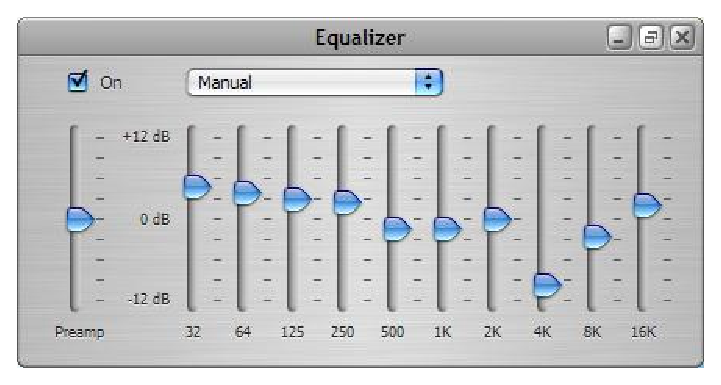
\includegraphics[width=0.7\textwidth]{equalizer}
   \caption{Ecualizador de reproductor de sonido. Cada barra deslizable controla la amplitud de cierto ancho de banda que se reproduce en el sonido.} 
 \label{fig:equalizer}
 \end{figg}
\end{figure}

De hecho, dado que la amplitud de cada frecuencia depende de la cantidad de agua en cada posición, la gráfica de frecuencia y amplitud después de la transformada de Fourier (es decir, el espectro) tendrá una forma muy similar al objeto mismo, como una proyección (Figura \ref{fig:proyeccionFrecuencia}).

\begin{figure}[htb]
 \begin{figg}
   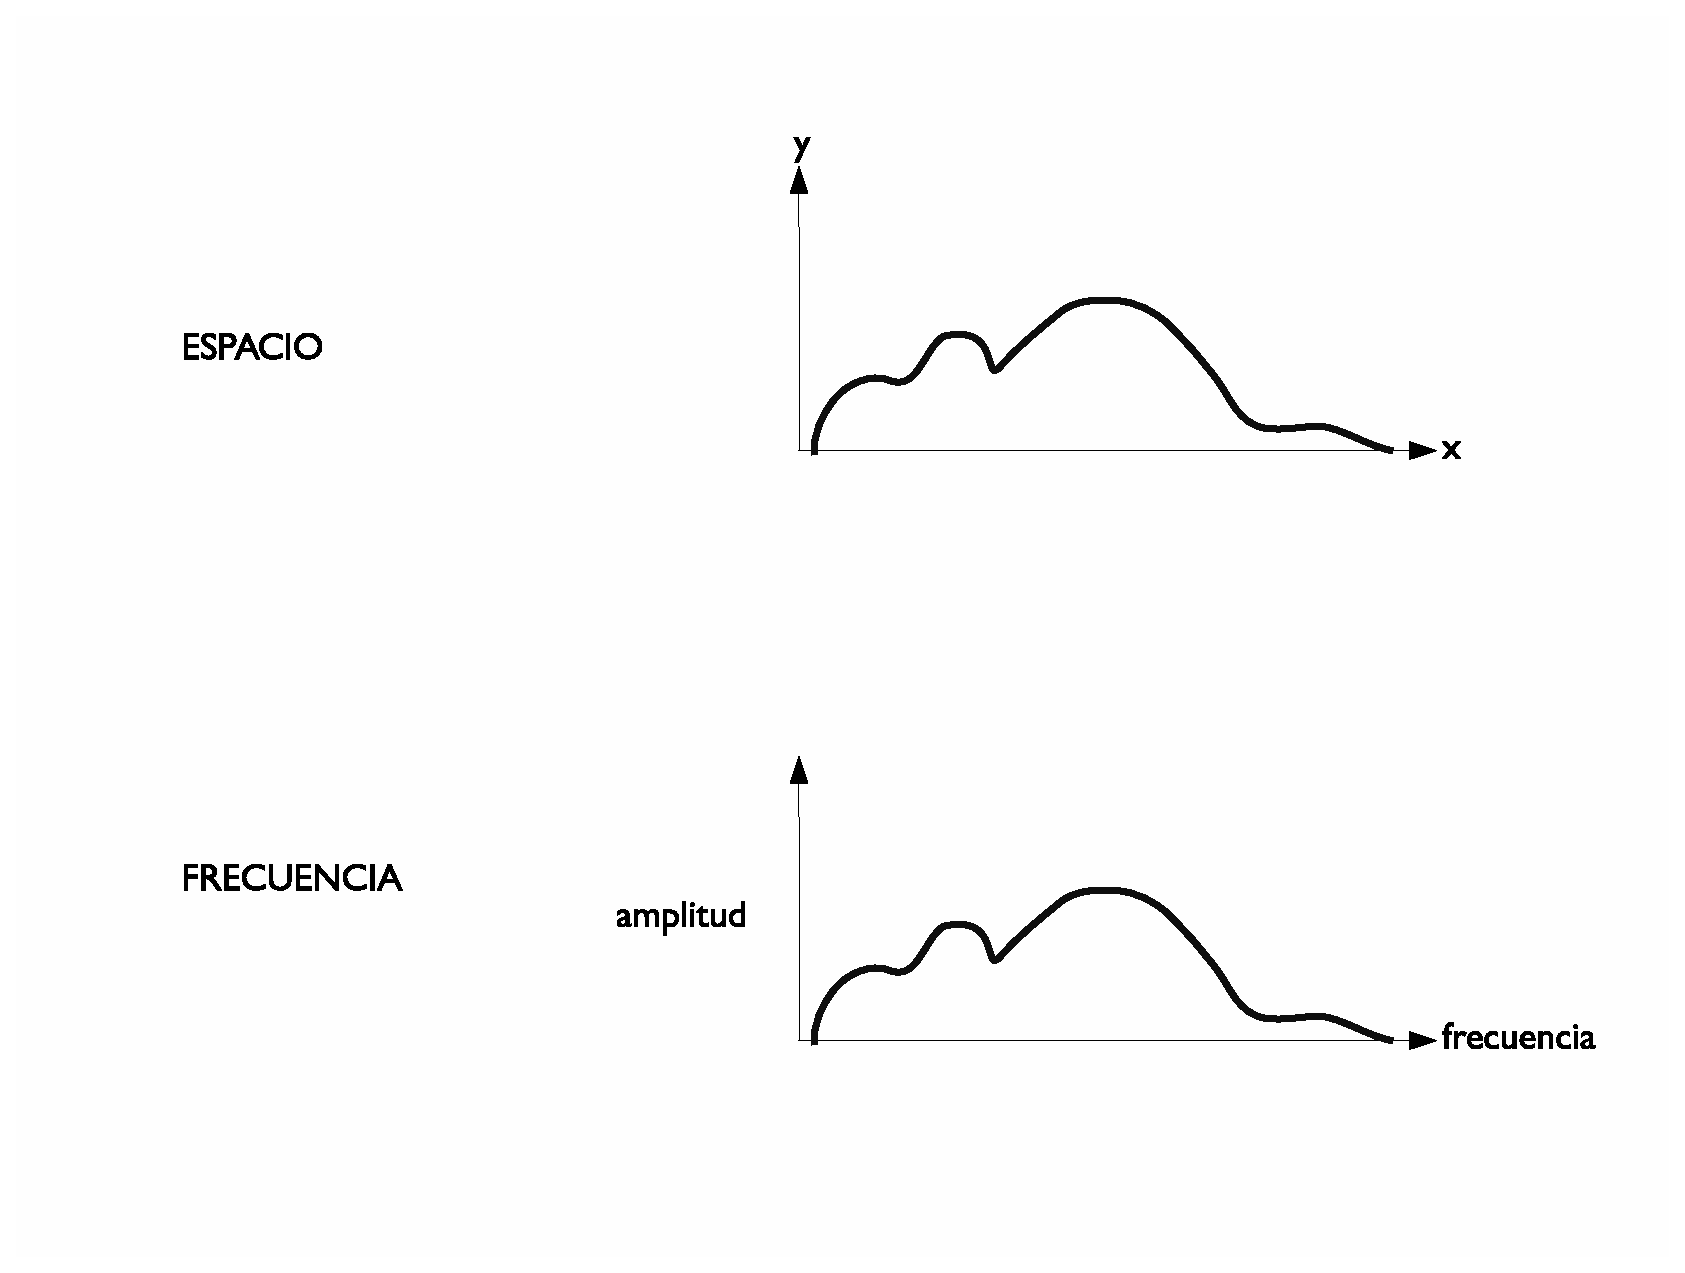
\includegraphics[width=\textwidth]{proyeccionFrecuencia}
   \caption{Proyección del objeto en el espacio de frecuencias. La amplitud de cada una de las frecuencias corresponde a la cantidad de agua presente en el objeto, que precesa a cierta frecuencia.}
 \label{fig:proyeccionFrecuencia}
 \end{figg}
\end{figure}


\section{Codificación mediante fase}
Las primeras dos dimensiones fueron fáciles de codificar: excitación selectiva y codificación por frecuencia y una simple transformada de Fourier. La dimensión que resta es menos intuitiva. Antes de abordar el tema, es importante mencionar que utilizando la codificación de frecuencia, y aprovechando el hecho de que la amplitud de cada frecuencia dibuja la proyección del objeto (Figura \ref{fig:proyeccionFrecuencia}), es posible realizar codificación de la última dimensión si se repite el experimento de codificación por frecuencia, pero cambiando la orientación del gradiente aplicado. En esta situación, la curva amplitud/frecuencia será la proyección del objeto visto desde distintas perspectivas dependientes de la orientación del gradiente. Si se acumulan suficientes proyecciones, se puede reconstruir la imagen en el plano mediante el método de retro-proyección (Funk-Radon) justo como en una tomografía. De hecho, ésta fue la primer técnica de codificación espacial de resonancia magnética, pero ha perdido terreno ante la codificación mediante fase.

Recordemos que una onda periódica (como una sinusoide) tiene tres características: su frecuencia (que es el inverso del periodo), su amplitud y su fase. Dos señales con frecuencia y amplitud idénticas pueden distinguirse si tienen fases distintas (Figura \ref{fig:fases}), y entendemos por fase el momento en que la amplitud pasa por el eje horizontal. La fase se describe en términos de radianes, o grados, pues las ondas sinusoidales son la representación lineal de un movimiento angular (Figura \ref{fig:sine_anim}).


\begin{figure}[htb]
 \begin{figg}
   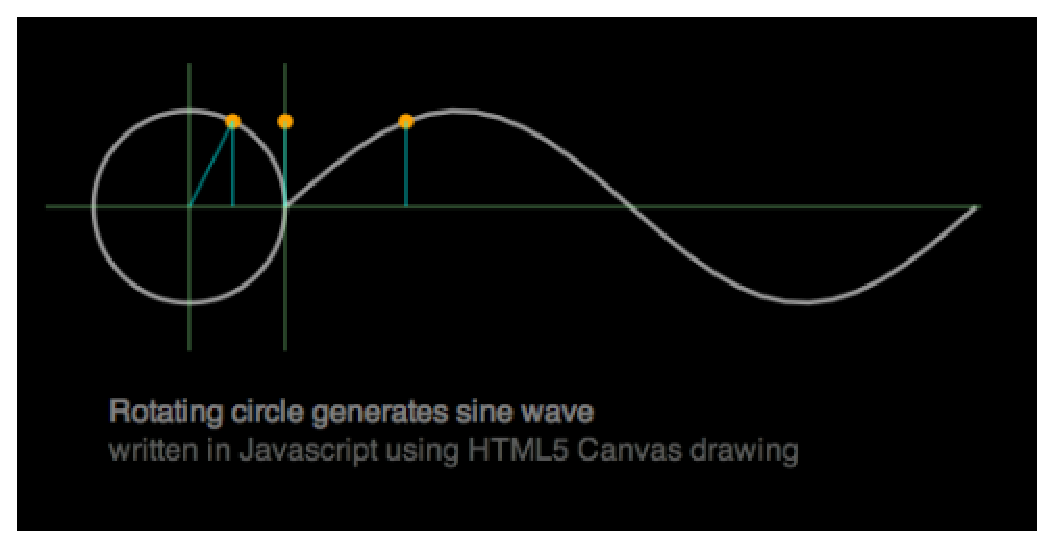
\includegraphics[width=0.7\textwidth]{sine_anim}
   \caption{Representación gráfica de la fase de un movimiento angular. Al rotar la línea radial en el círculo, su proyección sobre el eje de las $x$ representa el seno del ángulo creado. Este puede ser graficado linealmente (a la derecha). En caso de comenzar a graficar a diferentes ángulos, las curvas sinusoides tendrán la misma forma, pero comenzarán antes o después con respecto al eje $x$. Tomado de \url{https://quantblog.wordpress.com/2010/05/26/animated-sine-wave-in-javascript-html5}.}
 \label{fig:sine_anim}
 \end{figg}
\end{figure}

\begin{figure}[htb]
 \begin{figg}
   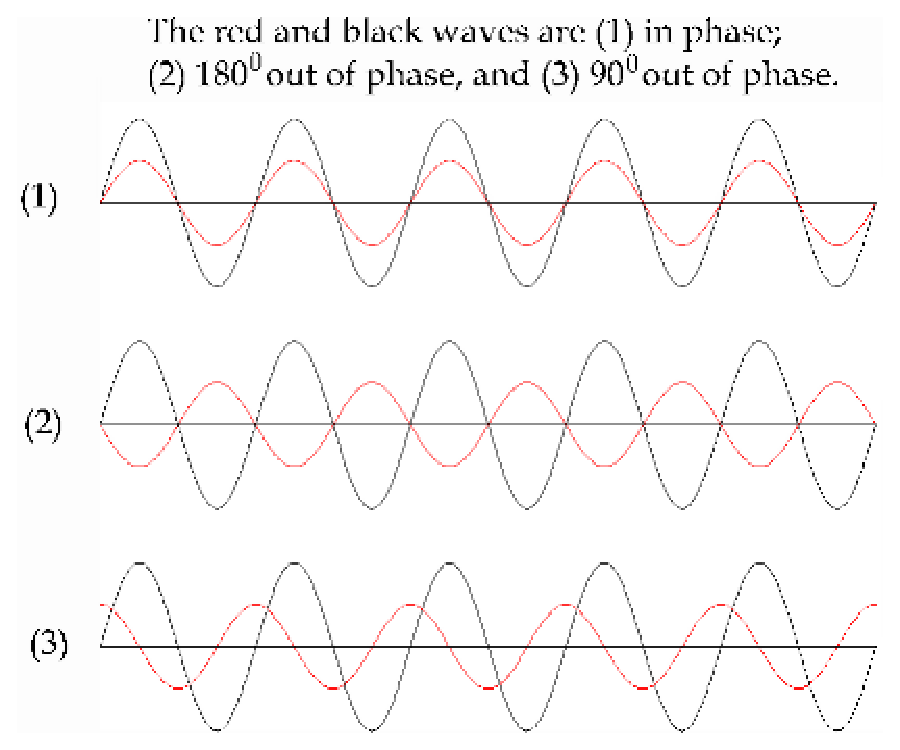
\includegraphics[width=0.7\textwidth]{fases}
   \caption{Tomado de \url{http://www.silcom.com/~aludwig/images/relphase.gif}}.
 \label{fig:fases}
 \end{figg}
\end{figure}

Dejaremos que la amplitud nos hable de la cantidad de agua, y quedó claro que la frecuencia nos puede hablar de una dimensión, así que permitiremos que la fase nos hable de la otra dimensión del plano. Con ésto podremos pasar de la proyección en una dimensión de un objeto, con el consecuente aplanamiento de la segunda dimensión, a la generación de la imagen completa. Si bien nuestra proyección amplitud/frecuencia seguirá siendo cierta, podemos obtener varias proyecciones, cada una con una fase distinta. 

Recordando que la frecuencia de precesión depende del campo magnético experimentado, podemos prender un gradiente del campo magnético  para otorgar distintas frecuencias en una dirección, pero al apagar el gradiente regresaremos a la frecuencia base, $\omega_0$, otorgada por \Bzero. Crucialmente, aunque tras apagar el gradiente todos los spins estén precesando a la misma frecuencia, habrá una diferencia entre sus fases en la dirección en que aplicamos el gradiente. La cantidad de fase que acumulan los spins ($\Delta\omega$) es proporcional a la magnitud del gradiente ($G$),  el tiempo ($t$) que se mantiene prendido y, por supuesto, la localización de los spins con respecto a este gradiente ($r$), de acuerdo a la ecuación \ref{eq_fase}:

\begin{equation}
 \Delta\omega = \gamma G(t) \cdot r
 \label{eq_fase}
\end{equation}


Es importante recalcar que el gradiente de fase debe prenderse y apagarse de manera independiente (habitualmente antes) del gradiente codificador de frecuencia, pues de lo contrario ambos gradientes se sumarían y modificarían de manera oblicua a \Bzero. Es también fundamental que las orientaciones de ambos gradientes sean perpendiculares entre sí. Así como en los problemas de matemáticas de educación secundaria, donde buscamos resolver tres incógnitas para lo que se requieren al menos tres ecuaciones, si queremos codificar el plano dividiéndolo en 128 posiciones verticales, necesitaremos repetir el paso de prender el gradiente codificador de fase al menos 128 veces, variando su amplitud de manera única en cada repetición, otorgando 128 fases distintas. 

La secuencia temporal en la que se juegan los diferentes componentes de excitación y codificación se conoce como \index{secuencia de pulsos} secuencia de pulsos. Recapitulando:

\begin{enumerate}
 \item Un pulso de RF excitador, simultáneo a un gradiente en una dirección ($z$, por ejemplo).
 \item Un pulso breve del gradiente codificador de fase, con cierta magnitud  (*).
 \item Un pulso codificador de frecuencia.
\end{enumerate}
(*) El paso 2 se repite tantas veces como se requiera para lograr mayor resolución, siendo la magnitud del gradiente distinto en cada paso. La señal que se recibe después de cada paso 3 posee distintas fases cada una, y se deben ir digitalizando y almacenando para posteriormente realizar una doble transformada de Fourier. El almacén de estas señales digitalizadas se conoce como \espaciok.


La extensión anatómica que se traduce en imagen se conoce como campo de visión, o más comúnmente como FOV (\emph{Field of view}) \index{FOV}, y tiene dos dimensiones más un cierto espesor de la rebanada. El usuario elige cuál de las dos dimensiones será codificada mediante frecuencia y cuál por fase. Asímismo, el usuario elige el número de particiones que tiene el FOV, lo que se traduce en la resolución de la imagen. Por ejemplo, el FOV puede dividirse en 128 columnas y 128 renglones. La resolución, entonces, se calcula simplemente:

\begin{eqnarray}
 Res_x = FOV_x / N_{frec}\\
 Res_y = FOV_y / N_{fase}
\end{eqnarray}
donde $Res_x$ y $Res_y$ son las dimensiones $x$ y $y$ de los pixeles resultantes, $FOV_x$ y $FOV_y$ son las dimensiones del FOV, y $N_{frec}$ y $N_{fase}$ es el número de particiones de las dos direcciones de codificación espacial. 

En el caso de la dirección codificada mediante frecuencia, cada pixel contiene un cierto rango de frecuencias (ancho de banda) que depende de la magnitud de $G$ y el FOV, de acuerdo a la ecuación \ref{eq_bw_read}. El total de las frecuencias en este ancho de banda se dividirá en el número de particiones del $FOV_{x}$. Si $G$ se mantiene constante y modificamos el número de particiones $N_{frec}$, el ancho de banda total no se modificará, pero sí lo hará en cada pixel. Es útil imaginar a cada pixel como un contenedor de diferentes frecuencias, y que cada pequeño paquete de frecuencias se asocia a una localización espacial. Lo anterior se aplica de forma idéntica a la dirección codificada por fase, con la particularidad de que cada uno de estos paquetes de frecuencias se logró mediante experimentos sucesivos en los que se modificó paulatinamente la magnitud del gradiente de fase.


Existen límites físicos y prácticos acerca de la máxima resolución alcanzable. Por ejemplo, la potencia máxima de los gradientes limitan la resolución, y siempre se debe recordar que mientras más pequeño sea el pixel, menos cantidad de moléculas de agua contendrá, lo que llevará a una degradación de la imagen resultante.


\section{El \espaciok}
\index{Espacio k|textbf}
\label{sec:espaciok}
Toda la información recibida por cada rebanada, en forma digital, se guarda en una matriz que tiene dos ejes: \kx y \ky. Las frecuencias aumentan de izquierda a derecha en el eje \kx y las fases en el eje vertical \ky. La matriz tiene tantas celdas celdas como el número de pixeles a reconstruir.  El nombre de este espacio se debe a que habitualmente se utiliza la letra $k$ para designar el número de periodos de una onda sinusoidal por unidad de distancia (habitualmente metros). Por ejemplo, una onda que presenta dos periodos en cada metro tiene una $k = 2 m^{-1}$.

Curiosamente, no existe una correspondencia punto a punto entre cada celda del \espaciok con cada pixel de la imagen. Por el contrario, cada celda del \espaciok contiene información de toda la imagen de manera simultánea, y cada pixel de la imagen está representado en todo el \espaciok. Cada celda $k_{x,i},k_{y,j}$ representa la amplitud de la frecuencia $i$ con fase $j$. La magnitud (intensidad) en cada celda del \espaciok indica qué tanto una cierta frecuencia y orientación está incluida en la imagen. En un ejercicio mental, podemos imaginar que ``pintaremos'' una imagen pero, en lugar de usar pinceles, usaremos una serie de sellos (o esténciles), todos de las mismas dimensiones (Figure \ref{fig:kspace_stencils}). Cada uno de estos sellos deja estampada una cierta frecuencia (cuántas rayas hay por cada cm, por ejemplo), y en qué orientación está dicha frecuencia (a cero grados, a 45 grados, etc). Algunos sellos los estamparemos fuertemente y con mucha tinta, mientras que otros los estamparemos con sutileza. En la medida en que los distintos sellos se sumen, emergerá nuestra imagen. El ejercicio anterior es análogo a lo que sucede en la corteza visual de los primates: existen neuronas que responden preferencialmente a barras luminosas con cierta frecuencia y orientación, y responden menos a otras frecuencias/orientaciones. Cada una de estas neuronas es un análogo de una celda del \espaciok.


\begin{figure}[htb]
\begin{figg}
   \includegraphics[width=0.6\textwidth]{kspace_stencils}
   \caption{Cada celda del \espaciok representa la intensidad con la que una cierta frecuencia y orientación está presente en la imagen (A-C). En D se muestra la suma de tres celdas del \espaciok. La totalidad del \espaciok se muestra en E, indicando las tres celdas cuya contribución a la imagen se muestran en A-C. La imagen resultante al utilizar todos los puntos del \espaciok de manera simultánea está en F (Mounsier Fourier, 1768-1830). }
 \label{fig:kspace_stencils}
 \end{figg}
\end{figure}



El \espaciok contiene dos juegos de señales: las codificadas mediante el gradiente de frecuencia (didácticamente $k_x$, aunque ésto es arbitrario), y las codificadas mediante el gradiente de fase (didácticamente $k_y$) (Figura \ref{fig:kspace_viz}). Lo único que resta para traducir en información espacial este conjunto de frecuencias es realizar la transformada de Fourier, que en este caso se realiza en dos dimensiones. Analíticamente, la transformada de Fourier es complicada y computacionalmente lenta, por lo que existen algoritmos que aceleran la obtención de las frecuencias que componen un grupo de señales complejas, siendo la más utilizada la transformada rápida de Fourier. Estos algoritmos suelen funcionar más eficientemente si las dimensiones del \espaciok son potencias de 2; esta es la razón por la que habitualmente las imágenes tienen un número de pixeles como 128\texttimes128 o 512\texttimes512.


\begin{figure}[htb]
 \begin{figg}
   \includegraphics[width=0.7\textwidth]{kspace_viz}
   \caption{Espacio $k$. Por cada codificación mediante el gradiente de fase se obtiene una señal (A). Cada señal es digitalizada y ordenada de acuerdo a la magnitud del gradiente de fase (B), y puede ser visualizada como una matriz de datos (B y D). Al unir los puntos en las columnas del \espaciok se obtienen las señales de la segunda dimensión, una por columna; se ejemplifica una de ellas en el panel C. Las líneas roja y negras en B y D representan las señales mostradas en A y C, respectivamente. D equivale a una vista superior de los datos presentados en B.}
 \label{fig:kspace_viz}
 \end{figg}
\end{figure}



Como se ve en la Figura \ref{fig:kspace_stencils}, el centro del \espaciok contiene información acerca de las bajas frecuencias espaciales (poca alternancia de negro/blanco a lo largo de la imagen real), mientras que las orillas del \espaciok tienen información acerca de altas frecuencias espaciales. Si obliteramos la información contenida en las orillas del \espaciok (convertimos los valores en cero) y realizamos la transformada de Fourier correspondiente, la imagen resultante será una versión borrosa de la original, pero se notará claramente que existen distintas estructuras con niveles de intensidad francamente diferentes (Figura \ref{fig:casos_espaciok}). Por el contrario, si obliteramos la información central del \espaciok, entonces veremos las estructuras de alta frecuencia espacial, es decir, los bordes de las estructuras de nuestra imagen, pero tendremos poco contraste entre estructuras. Además, existe una simetría conjugada en los ejes vertical y horizontal de este espacio, por lo que parece que se mirara a sí mismo en el espejo. Esto da características singulares al \espaciok que pueden ser explotadas ampliamente. Por ejemplo, es posible generar una imagen a partir de poco más de la mitad del \espaciok, lo que significa que podemos obviar la necesidad de adquirir cada uno de sus renglones, lo que nos ahorraría tiempo en la adquisición de la imagen; en efecto, esta es una técnica muy utilizada en la práctica diaria. Por otra parte, algunos algoritmos de compresión de imagen (JPEG, por ejemplo), utiliza esta estrategia para reducir la cantidad de información que se almacena en el disco, sufriendo mínimas consecuencias en la imagen reconstruida a partir de esta información parcial.


\begin{figure}[htb]
 \begin{figg}
   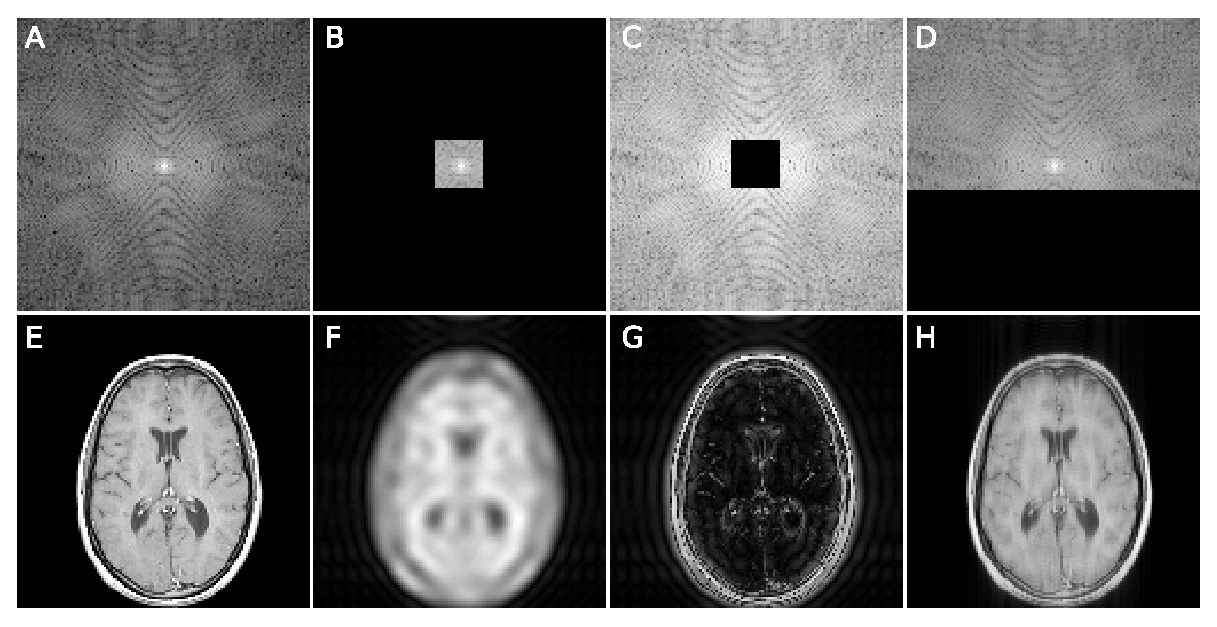
\includegraphics[width=\textwidth]{casos_espaciok}
   \caption{Características del \espaciok. En A se presenta la totalidad del \espaciok correspondiente a la imagen del panel E. A los datos presentados en A se les convirtió a ceros artificialmente su información contenida en toda la periferia (B), lo que genera una imagen con alto contenido de contraste, pero difusa (F). El ejercicio reverso (C) muestra que la periferia del \espaciok guarda la información relativa a los bordes de la imagen (G). Por último, poco más de la mitad del \espaciok (D) es suficiente para reconstruir la imagen con poca degradación (H).}
 \label{fig:casos_espaciok}
 \end{figg}
\end{figure}


Siguiendo la manera en que postulamos previamente, el \espaciok se llena línea por línea, o unas cuantas líneas por vez. Como se verá en el capítulo \ref{chapter_secuencias}, existen varias formas de llenar el \espaciok, no necesariamente cartesianas.







